%%
%%
%%      SECTION: BEAM PATTERN 
%%

%% [intro]
%%________________________________________________________

The NIKA2 beam pattern mainly depends on the IRAM 30m telescope and
NIKA2 full (external and internal) optical system characteristics,
whereas the detectors themselve might have an impact at sub-dominant
level (through e.g. time constants or correlated noises).

In this section, we characterize both the main beam, which is
modeled as an elliptical Gaussian, and the full beam pattern including
error beams up to angular scales of 10 arcmin.



%% [Full beam pattern]
%%________________________________________________________
\subsection{Full beam pattern}
\label{se:fullbeam}

\subsubsection{Data sets}
\label{se:beammap_set}

The characterization of the IRAM 30-m beam pattern observed through NIKA2 detectors is mainly based on observations of strong compact sources, such as planets including Uranus, Neptune and Mars, and bright quasars. We generally use beam-map scans, which we recall, are deep-integration raster-scan observations that consist of 99 sub-scans placed at intervals of $4.8''$ to cover a total of $13.5' \times 7.8'$. Most of our beam-related analysis are beased on the same set of beam-map scans as previously selected to perform the average FOV reconstruction. The set comprises nine beam-map scans that distribute as one from N2R8, '20170125s243', two from N2R9, '20170224s177' and '20170226s415' and six from N2R10, which are '20170226s425', '20170227s84', '20170419s133', '20170420s113', '20170424s116', '20170424s123'. 


\subsubsection{Deep beam maps}
\label{se:beammaps}
We present the two-dimensional distribution of the beam in Fig.~\ref{fig:beam}. We primary use a map obtained from a combination of deep observations of strong point sources collected during \emph{NIKA2-run8} and \emph{run9}. Namely, we use 'beammap' OTF scans of Uranus (scan id '20170125s223' and '20170125s243'),  Neptune ('20170224s177') and the bright quasar 3C84 ('20170226s415'). However, we checked the stability of our results on single scan maps, combinations of scans for a single source, and combinations of shallower scans but spanning a large range of scanning direction. The data processing includes a mitigation of the correlated noise, which mainly originates from the atmosphere.  We primarly use a subtraction of a common mode estimated from the most correlated detectors (the so-called 'cm one block' method). However, other methods are tested for assessing the immunity of our results to noise residuals.

\begin{figure}
\begin{center}
  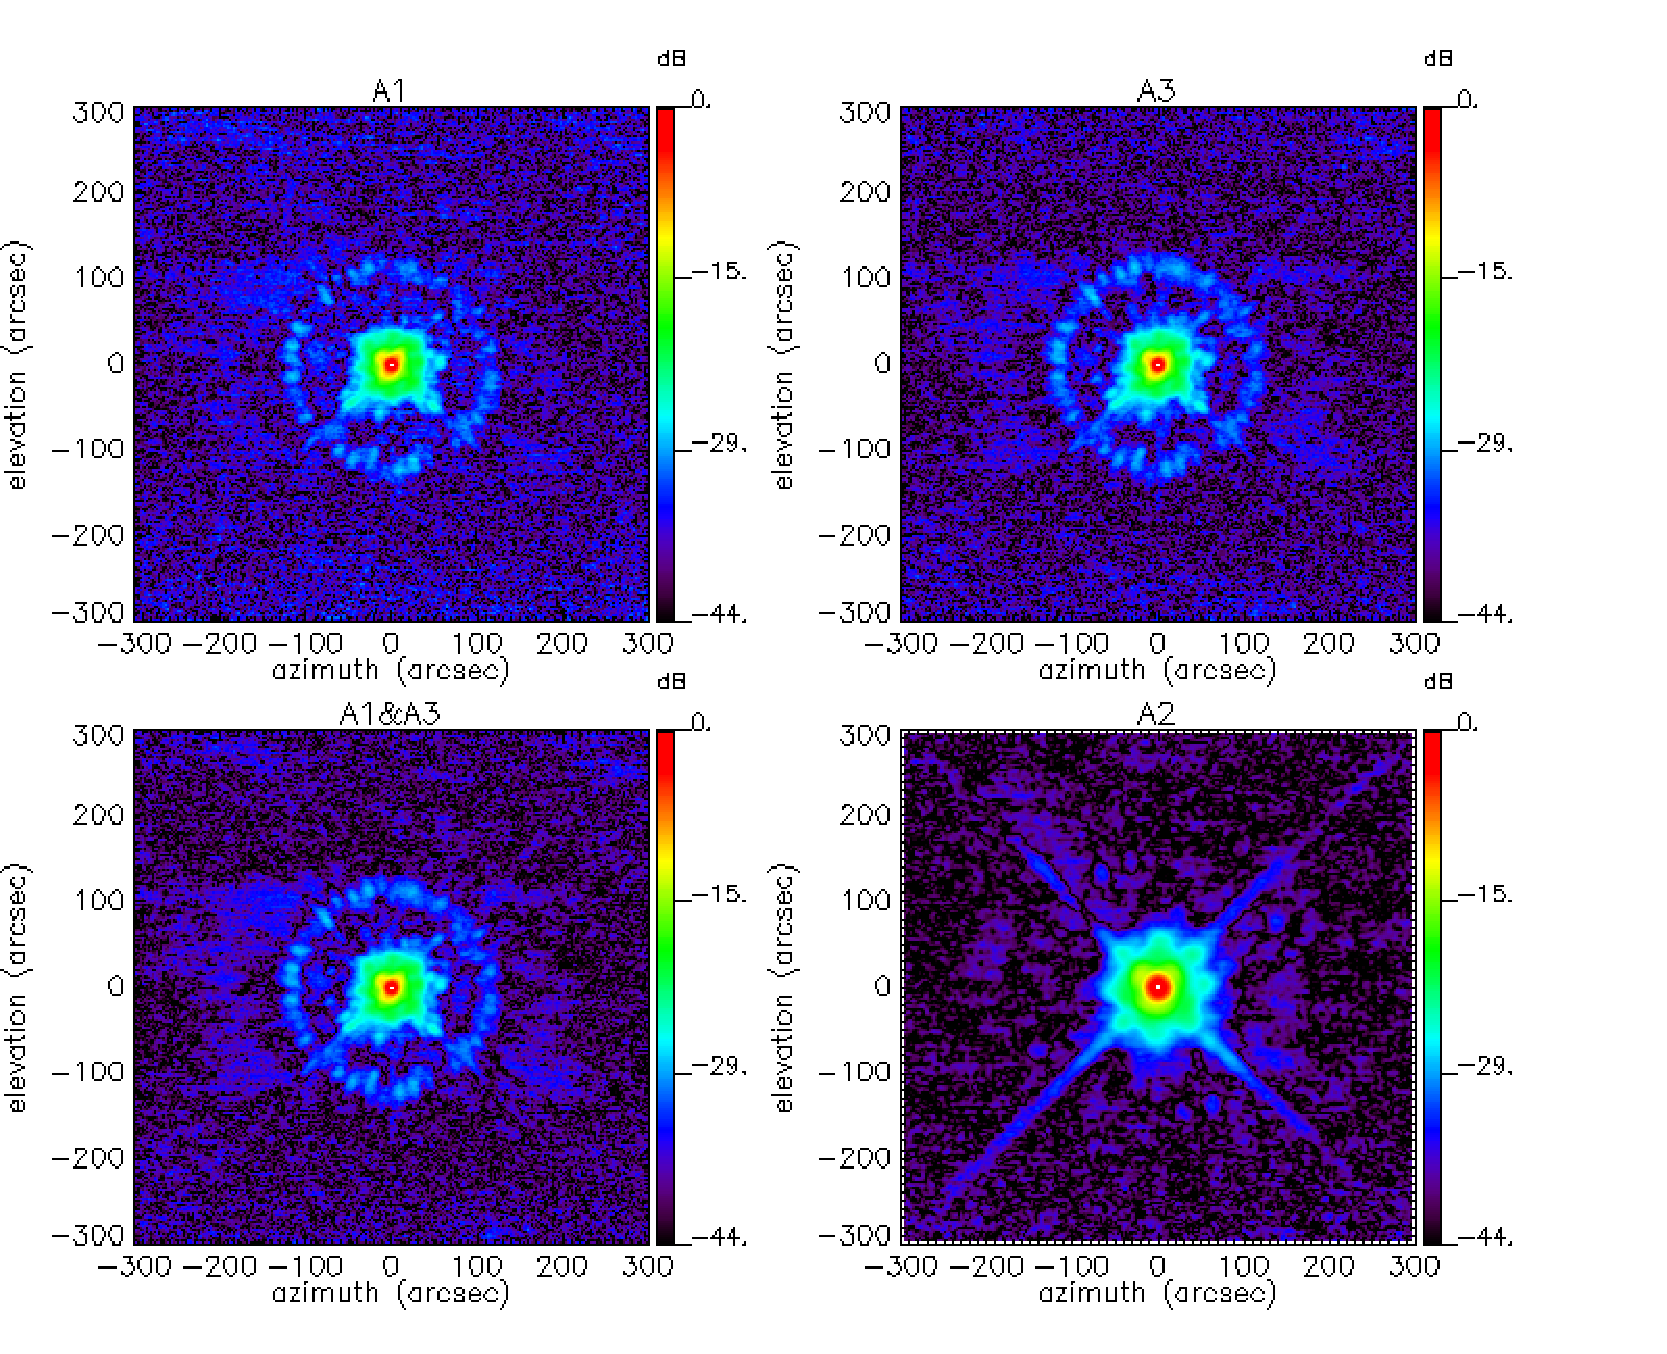
\includegraphics[clip, angle=0, scale=0.4]{Figures/Lobe_map_Combo_v2_dB.pdf}
 \caption{Beam pattern. From upper left to lower right, beam maps of array 1 (labeled 'A1'), array 3 ('A3'), the combination of the 1.15mm arrays ('A1$\&$3') and the 2mm array ('A2') are shown in decibel. These maps, which consist of normalized combination of four long OTF scans of bright point sources, are in celestial coordinates and cover a sky area which extend over 10 arcmin.}
\label{fig:beam}
\end{center}
\end{figure}


The deep NIKA2 beam maps reveal some noticeable features, which are
shown in Fig.~\ref{fig:features}.

{\bf Implement Samuel's comments copied below}
Commentaires faits � Alessandro pour le papier:
\begin{itemize}
\item[(1)] les four symmetrical spokes of the error beam sont normaux
  et attendu d'apr�s mes simus comme tu peux voir dans la petite image
  ci-dessous (c'est le beam obtenu dans Zemax pour la bande 1mm
  convolu� avec une fonction porte de la taille du pixel)
\item[(2)] par contre les pink ellipse show spikes in this map
  montrent un effet de diffraction ou de ghost image anormal et
  inattendu qui est du \'a un probleme optique dans le cryostat ou au
  niveau de M5 ou M6 ou la fenetre. On le sait car quand on regarde
  leur position en fonction de l'elevation on voit qu'ils tournent
  avec l'elevation dans les cartes Az-El
\item[(3)] quant aux spikes of unknown origin montr\'es sur A3 je pense
  que les deux en bas et � droite sont juste un des petits lobes de la
  simu avec un meilleur contraste que ceux du haut et de gauche, alors
  que pour le petit blob dans la diagonale a peu pres au niveau de
  la diffraction sur un bras du quadrupode je soup�onne un effet
  d'amplification du a la petite boite qui se trouve sur le cot\'e du
  secondaire que tu peux voir sur la photo du slide 2 de la
  presentation qu'Andrea a envoyee aujourd'hui (mais je n'ai pas de
  preuve)
\end{itemize}



\begin{figure}
\begin{center}
  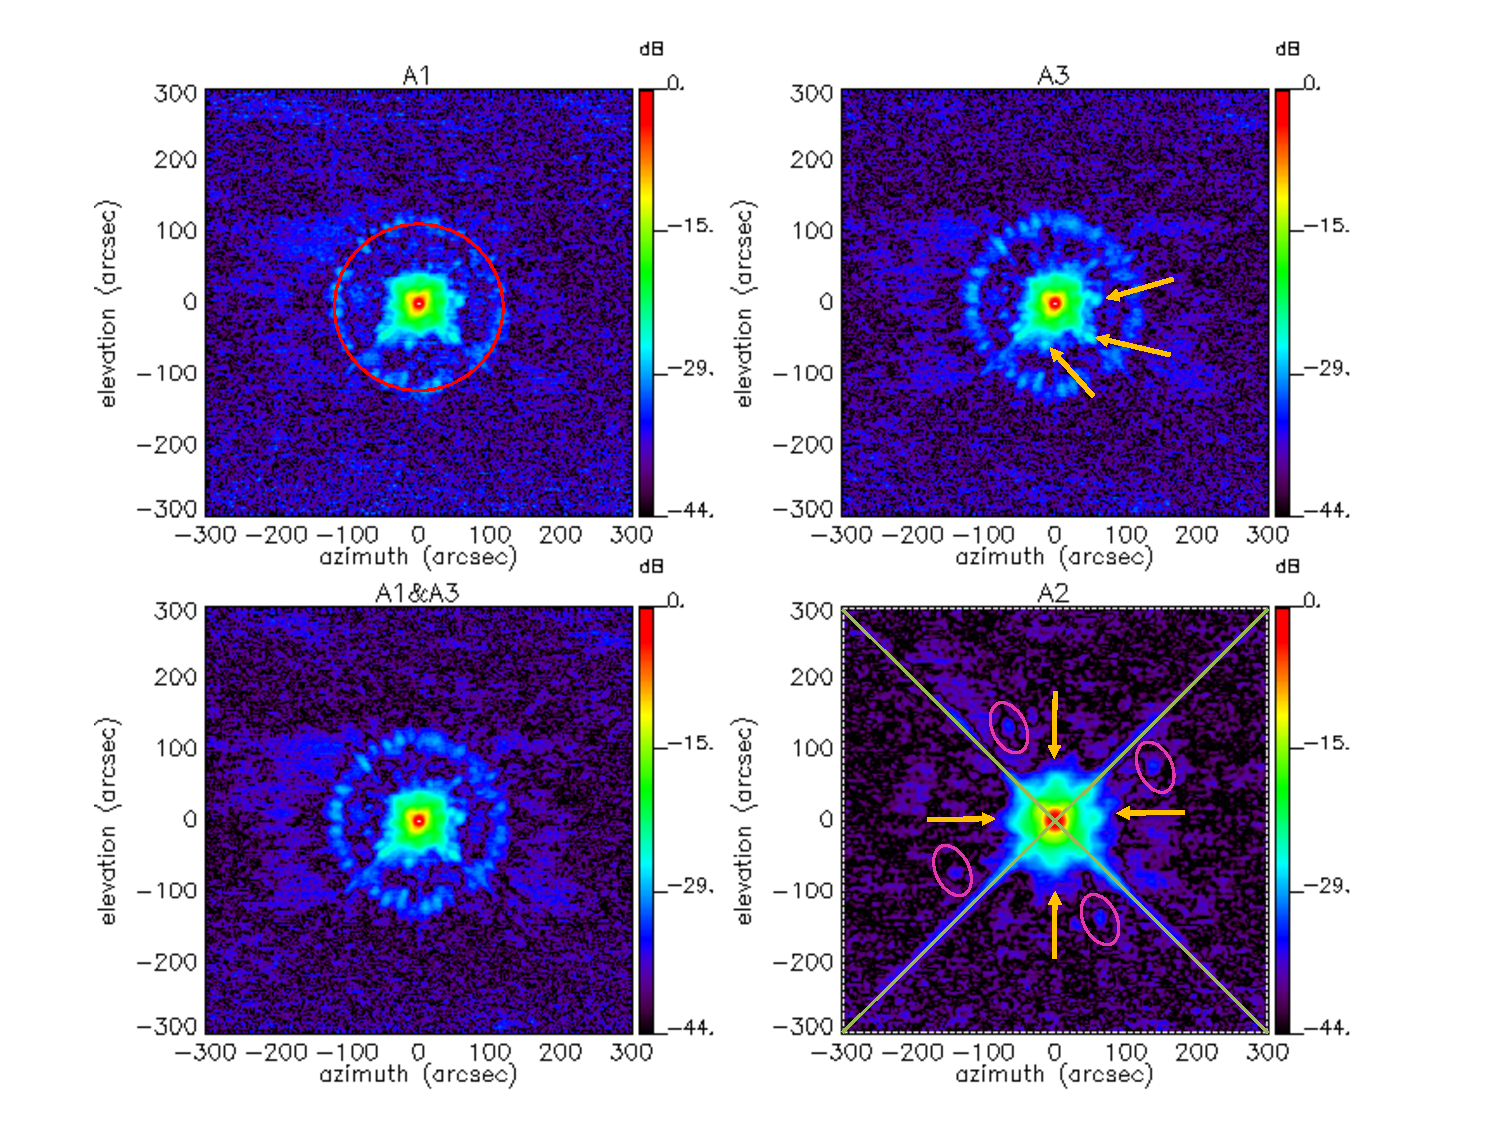
\includegraphics[clip, angle=0, scale=0.4]{Figures/Beams_features.pdf}
\caption{Noticeable features of NIKA2 beam pattern. Red circle: diffraction ring seen in 1-mm maps (the spokes are presumably caused by radial and azimuthal panel buckling (cf. Fig.4 in Greve et al. 2010)); Perpendicular green lines: diffraction pattern caused by quadrupod secondary support structure (prominently seen in 2mm maps); Yellow arrows in the upper right pannel: pattern of 3 spikes seen in 1mm maps of unknown origin; Yellow arrows in the lower right pannel: four symmetrical spokes of the first errorbeam; Pink ellipses: 4 spikes seen in 2mm maps.}
\label{fig:features}
\end{center}
\end{figure}


To gain a first impression of the structure of the Iram 30-m beam as seen with NIKA2, we use radial cuts to evidence the relative level of the main beam, the first error beam and other features seen in the 2D beam pattern using radial cuts. NIKA2 full beam is shown in Fig.~\ref{fig:beam_db} by means of two orthogonal cuts through Uranus
from a high quality map obtained on 2017 January 25th in excellent conditions
(low opacity $\tau_{225}=0.08$ and elevation $46^{\circ}$).

\begin{figure}[h]
\begin{center}
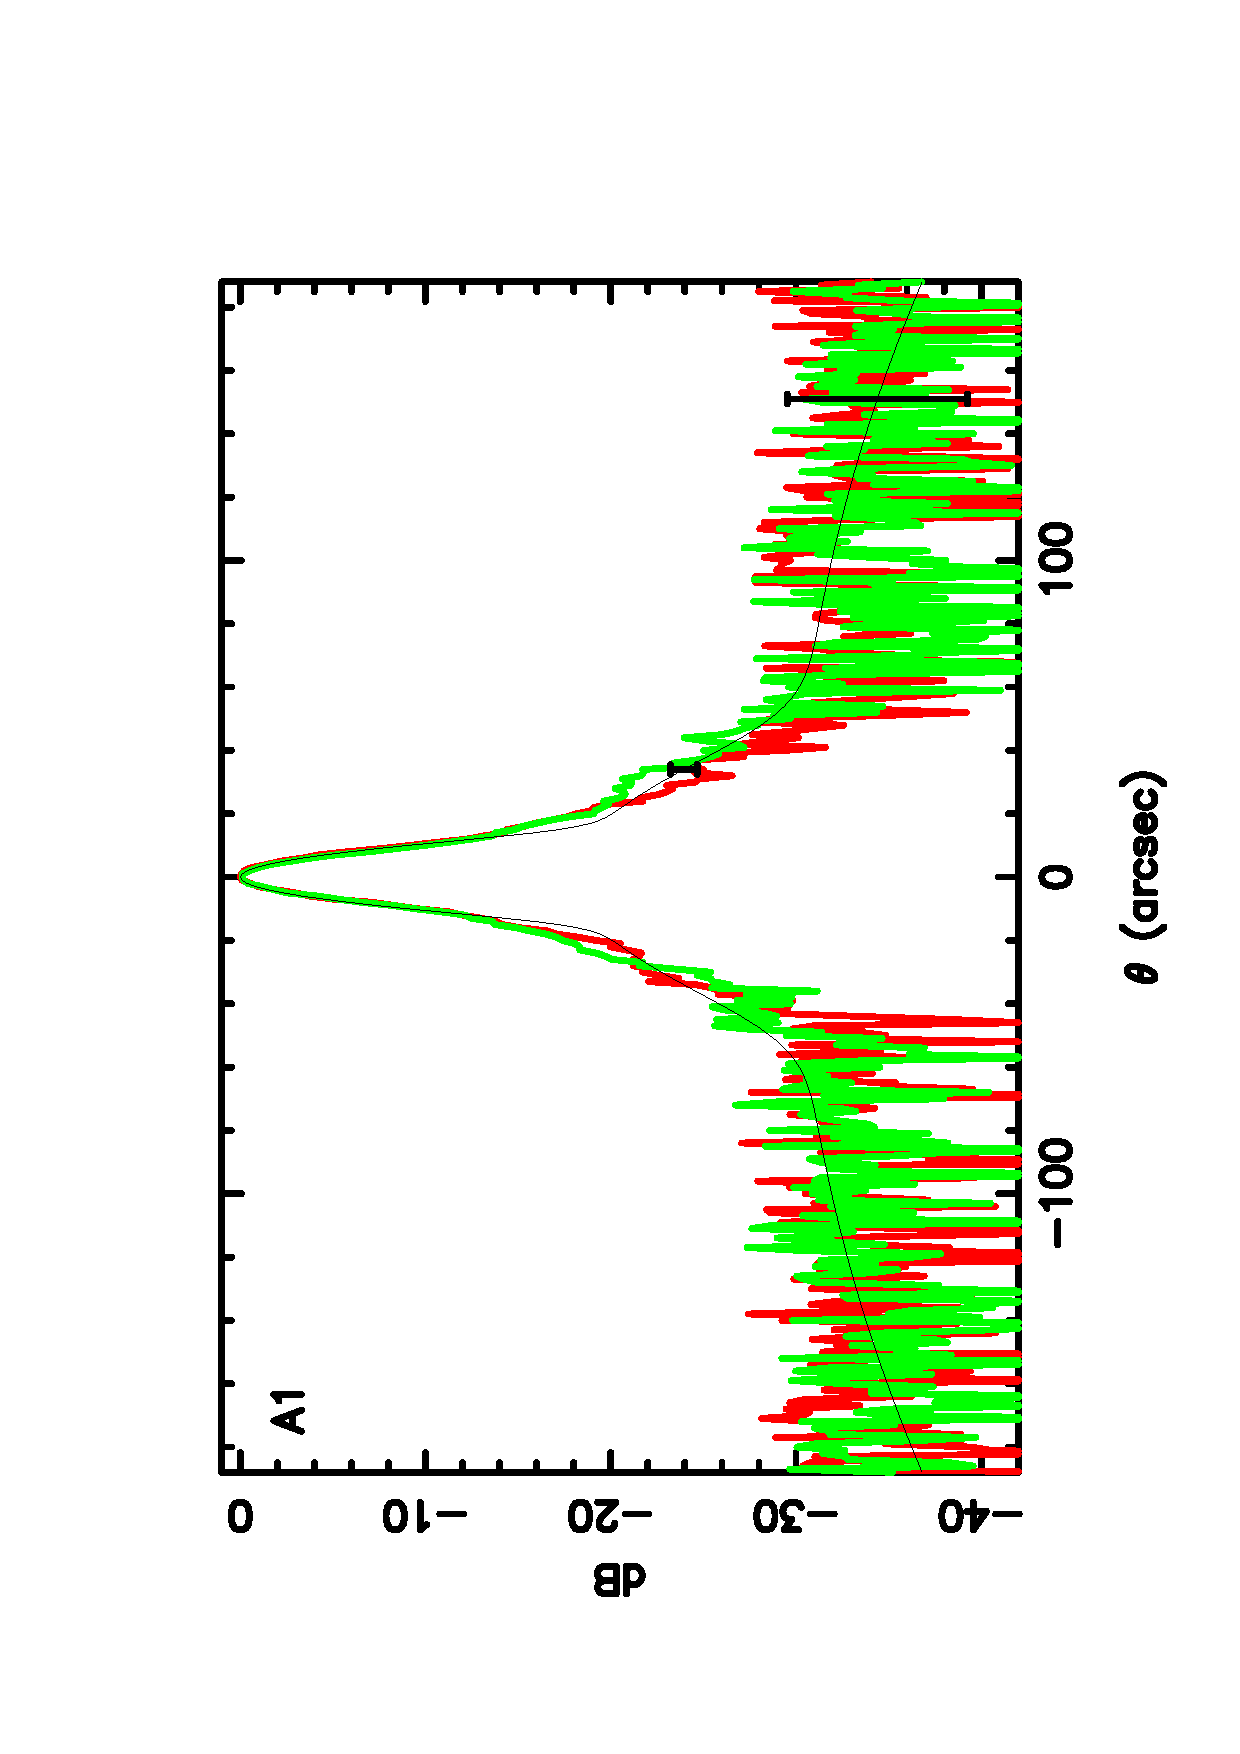
\includegraphics[clip, angle=-90, scale =0.3]{Figures/Array_A1_dB.pdf}
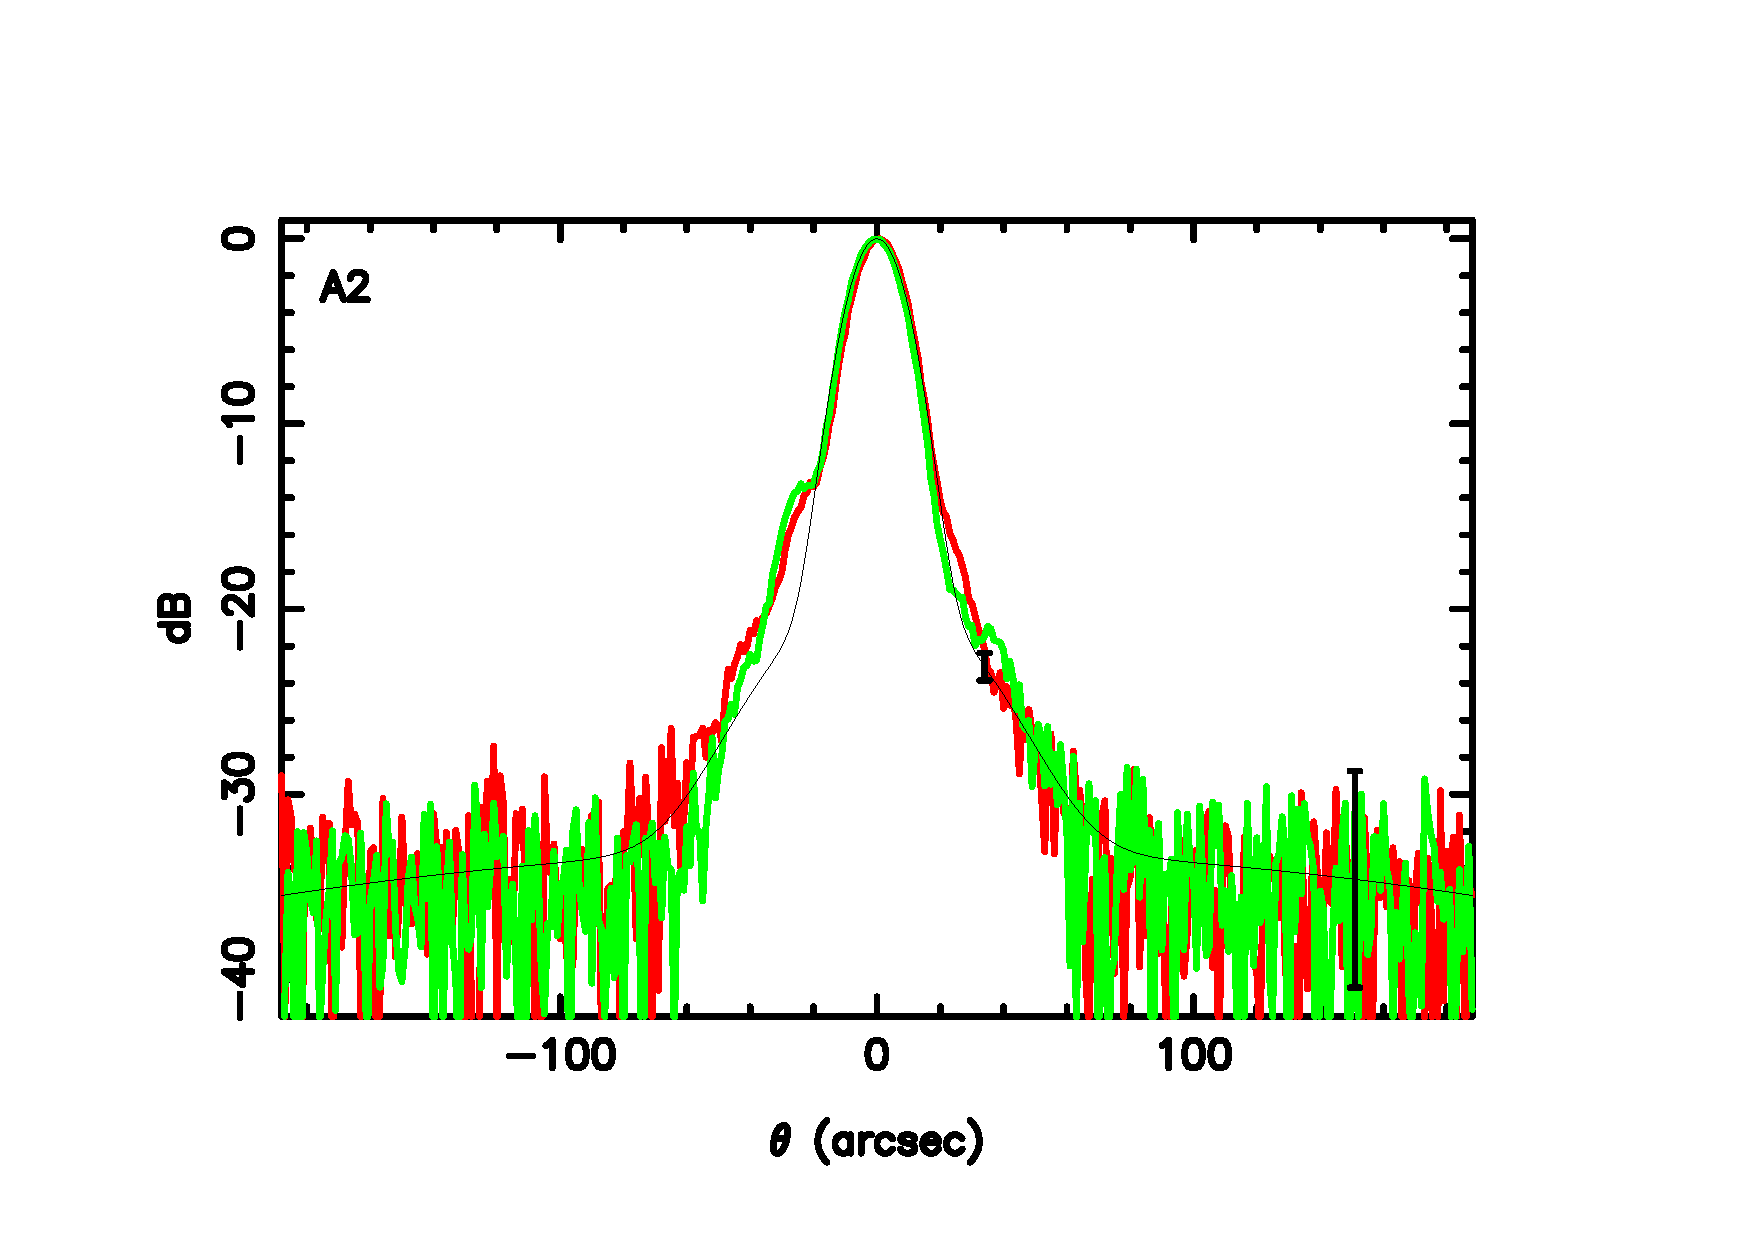
\includegraphics[clip, angle=-90, scale = 0.3]{Figures/Array_A2_dB.pdf}
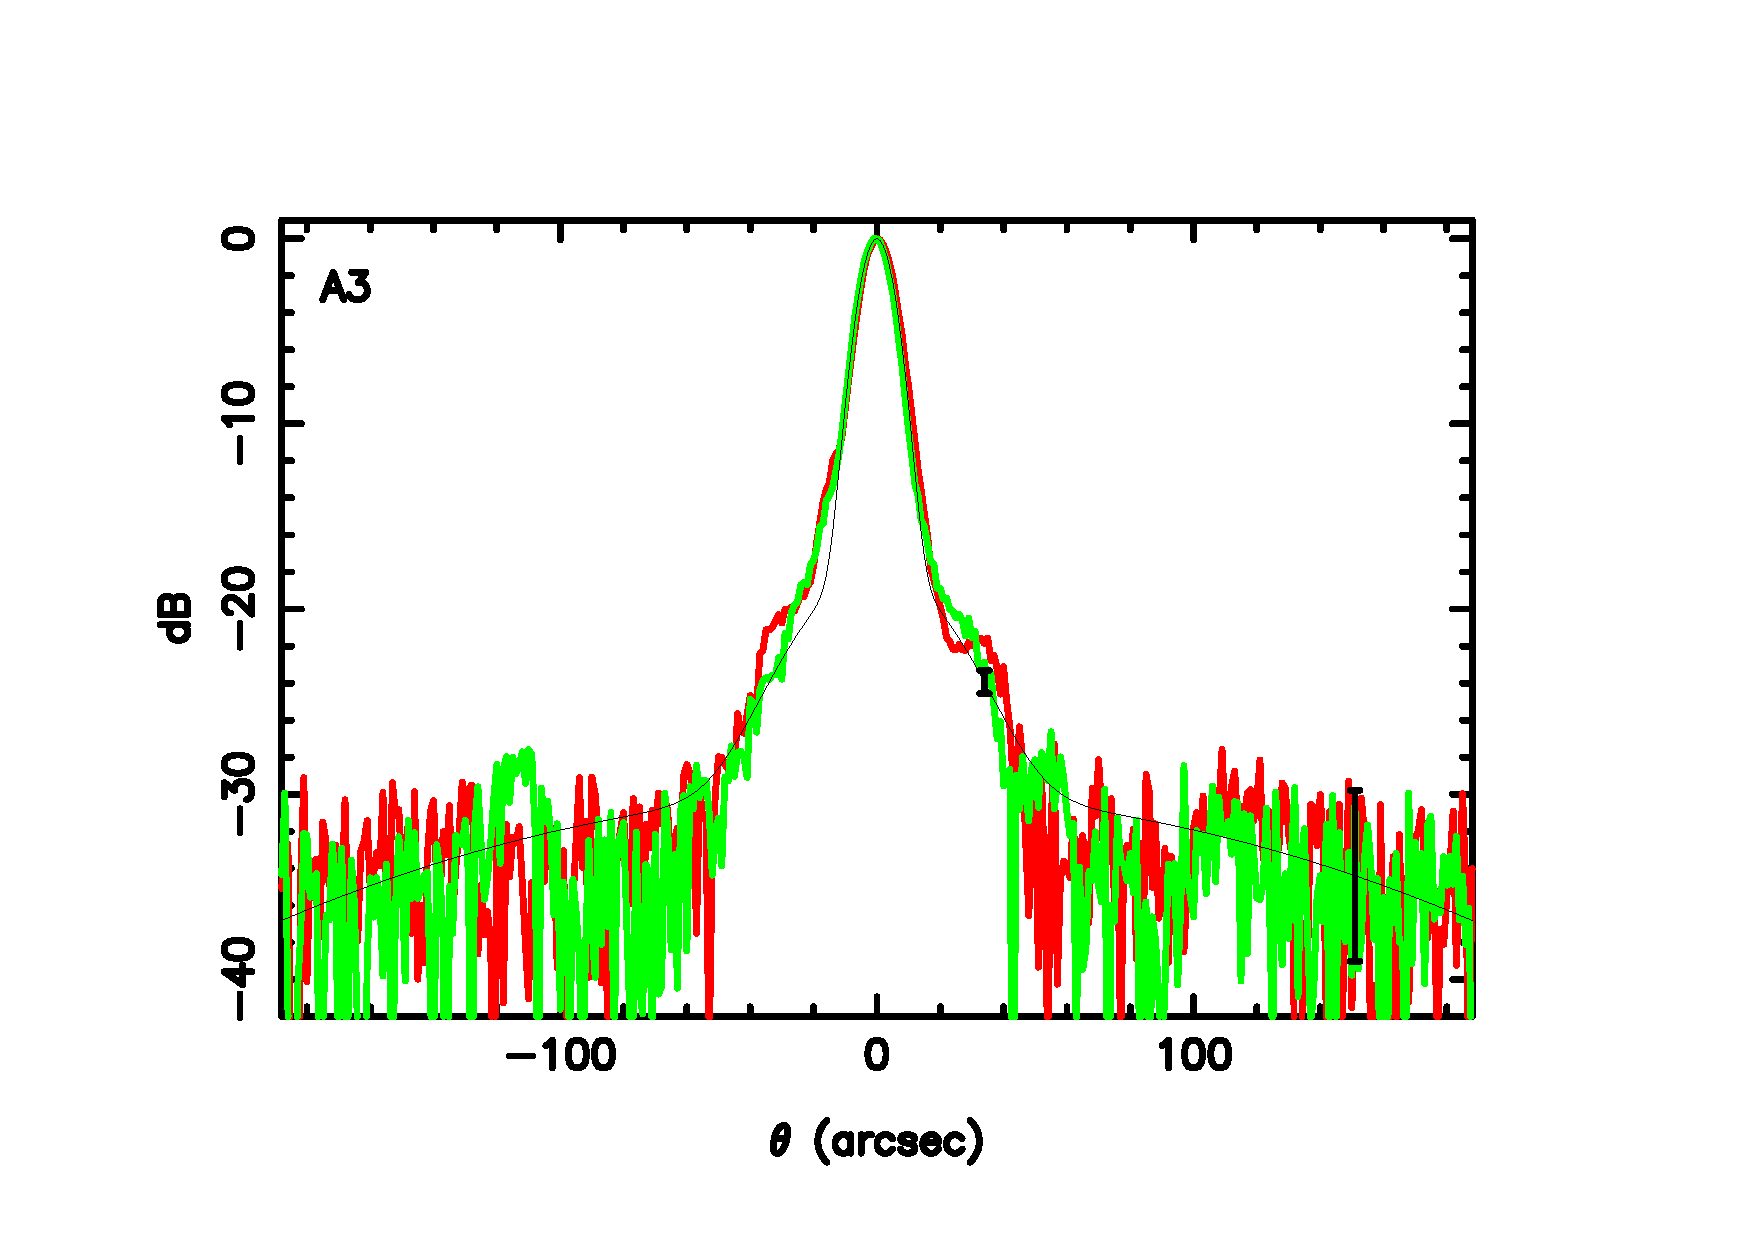
\includegraphics[clip, angle=-90, scale = 0.3]{Figures/Array_A3_dB.pdf}
\caption{Two orthogonal cuts through the beam are shown in red and green and a best fit model made
of three Gaussians is superimposed in black. These cuts were obtained from the high quality map of Uranus on 2017 January 25th.
The main beam starts to depart from the first Gaussian at -12dB. }
\label{fig:beam_db}
\end{center}
\end{figure}

A model made of three Gaussians centered on the source peak was best
fit {\it by hand} to these cuts.
%the parameters are reported in Table \ref{tab:3gauss} [PEUT-ETRE
%AVANTAGEUSEMENT REPLACED PAR VALEURS DE FLORIAN].
We observe that the main beam starts to depart from the first
Gaussian at the level of about -12dB for the three arrays.
We note that for the instrument EMIR on the radiotelescope,
this departure is about -20dB (Kramer, Penalver and Greve
2013). However, this
discrepancy between a feedhorn-based experiment and a bare pixels one
is expected since the main effect of the feedhorns is to lower the
side lobes of the Airy diffraction pattern.
The precise characterization of the full beam structure is discussed
in Sect.~\ref{se:fullbeam_prof}.  

%From parameters in Table \ref{tab:3gauss}, one can estimate that
%the source incident power is split about equally between the main beam
%and the error beam at 1mm, and these fractions are 70\% and 30\% at 2mm, respectively.
%This modelling uses the central
%region   $180'' \times 180''$ in size with a uniform noise rms from
%a larger area of 8' x 5' on the sky scanned with the arrays. It is expected
%that the error beam extend beyond these limits.


%\begin{table}
%\centering 
%\caption[]{Model parameters of the three Gaussian beam.}
%\begin{tabular}{|l|l|l|l|l|l|l|}
%\hline
%               & \multicolumn{3}{c|}{A1 and A3} & \multicolumn{3}{c|}{A2}  \\
%\hline
%fwhm      & $11.25''$ & $45''$  & $250''$ & $17.75''$ & $56''$  & $420''$ \\
%amplitude & 0.984     & 0.015   & 0.0005   &  0.9875   & 0.011   &  0.0005\\
%\hline
%\end{tabular}
%\label{tab:3gauss}
%\end{table}


\subsubsection{Beam profile}
\label{se:fullbeam_prof}

{\bf complete this sub-section}

The beam profile is the azimuthal average of the beam map around the
main beam center. Although the profile cannot represent the sub-dominant non-axisymetrical
extended features, which are seen in the beam pattern and discussed in
Sect.~\ref{se:beammaps} (telescope arms, spikes), it provides us with a useful
representation of the internal and central parts of the beam (about up to
$100''$). We determine a beam profile from a beam map in centering to
the fitted value of the main beam center and forming the
weighted average of the pixels equidistant to the center.

We model the beam profile as a three-Gaussian function defined as:
\begin{equation}
  B(\theta) = \sum_i A_i G_i(\theta) + B_0
\end{equation}


Figure \ref{fig:beam_profiles_3G} shows the beam profile from a beam
map acquired during {\emph N2R8} (scan ID: 20170125s223), as well as
the best-fit 3-Gaussian model. 

\begin{figure*}[h!]
\centering
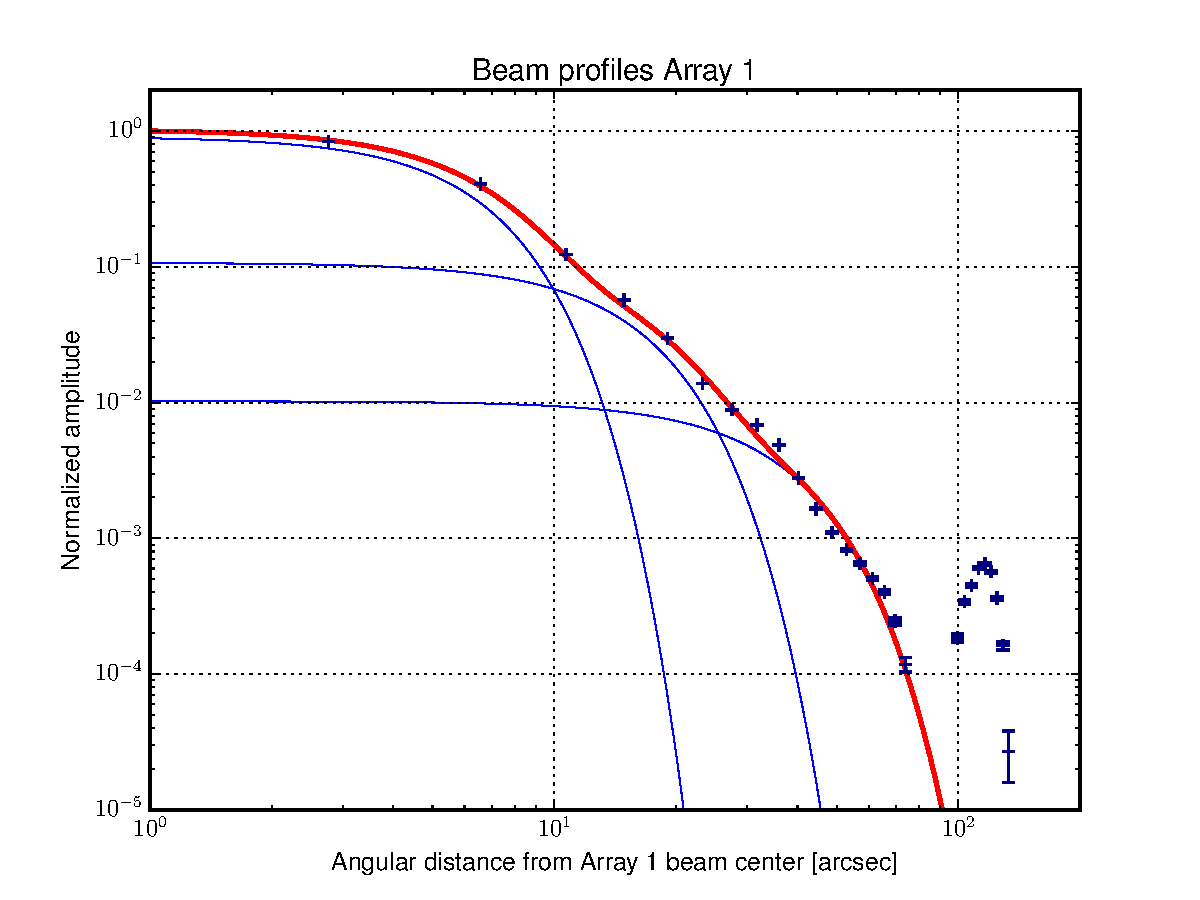
\includegraphics[height=6cm]{Figures/Beam_profiles_A1_FR.pdf}
\hspace{0.5cm}
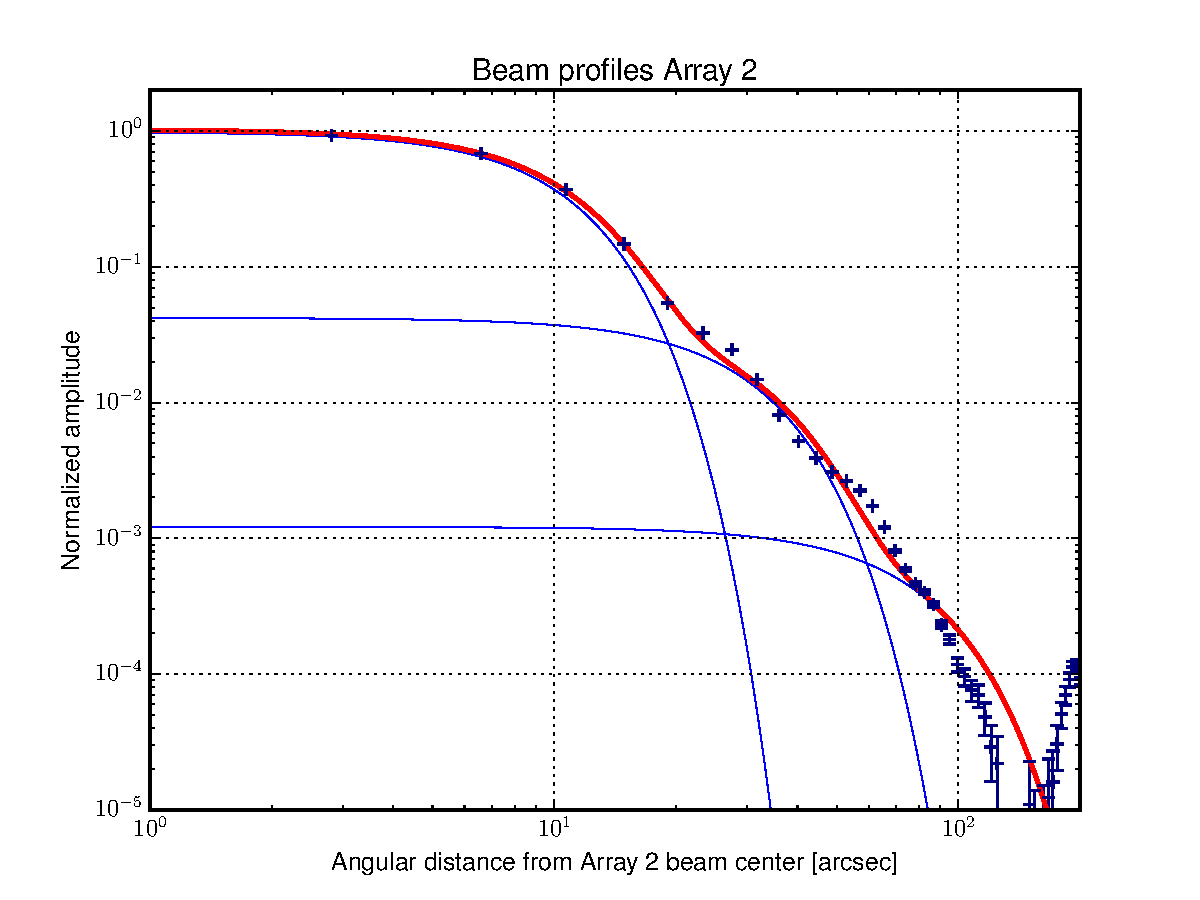
\includegraphics[height=6cm]{Figures/Beam_profiles_A2_FR.pdf}
\hspace{0.5cm}
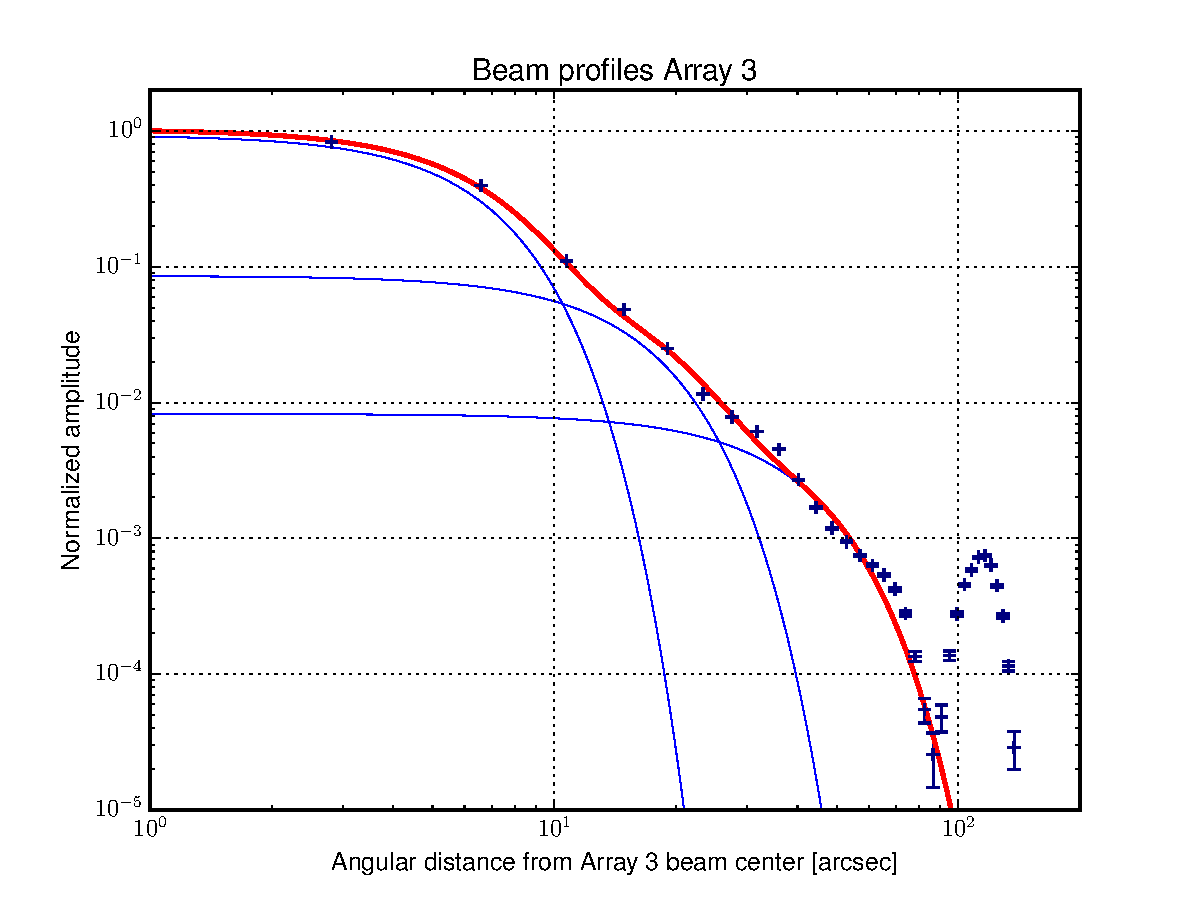
\includegraphics[height=6cm]{Figures/Beam_profiles_A3_FR.pdf}
\caption{{\footnotesize Beam profiles for array 1, 2, and 3.}}
\label{fig:beam_profiles_3G}
\end{figure*}



%% [Main beam]
%%________________________________________________________
\subsection{Main beam}
\label{se:MB}


We define NIKA2 main beam as the principal Gaussian (of the smaller FWHM)
that encloses most of the meassured source flux. The principal-power,
smaller-FWHM Gaussian fitted function within the three-Gaussian model,
as discussed in Sect.~\ref{se:fullbeam_prof}, provides us with a first
estimate of the main beam, which is given in Table~\ref{tab:fwhm}. However,
this estimate could be biased toward the lower-FWHM values due to
degeneracies between the three-Gaussian model parameters. To ensure
obtaining robust main beam FWHM estimates, we devise two alternative dedicated
methods, which both resort to masking the side lobes: i) Gaussian
fits of the beam profile to benefit from the signal-over-noise
increase after azimuthally averaging the signal, ii) Elliptical
Gaussian fits of the beam map for a better 2D modeling. Cross-checking
the outputs from these complementary methods is an important robustess
test of our results.

We also consider different data sets acquired during \emph{N2R8}, \emph{N2R9}
and \emph{N2R10}: i) a series of $8' \times 5'$ OTF
scans of primary and secondary calibrators, ii) beam-map scans of
Planets.

Table~\ref{tab:fwhm} gathers the main beam FWHM results obtained using the three
discussed methods and two datasets.  


\subsubsection{Sidelobe-masked Profile-based analysis}

{\bf add a description here [Jean-Francois's method]}

\subsubsection{Sidelobe-masked Map-based analysis}

\paragraph{Method description}

NIKA2 main beam two-dimensionnal distribution is modeled using an elliptical Gaussian. We characterize NIKA2 resolution by giving the \emph{FWHM}, defined as
\begin{equation}
  FWHM = 2 \sqrt{2\ln {2}} \sqrt{\sigma_x\sigma_y},
\end{equation}
where $\sigma_x$ and $\sigma_y$ are the Gaussian standard deviation along minor- and major-axis. To avoid the side lobes contamination, we use masked versions of the beam map, in which an annulus of inner radius $r_{\rm{in}}$ and outter radius $r_{\rm{out}}$ is cut out. Whereas $r_{\rm{out}}$ is conservately set to be $100 arcsec$, $r_{\rm{in}}$ is let free to vary around a central value about $8'$ for A1 and A3 and about $12'$ for A2 to provide the best 2D Gaussian fit.  

\paragraph{Estimates using $8' \times 5'$ OTF scans}

We select \emph{N2R9} and \emph{N2R10} $8' \times 5'$ OTF scans of
bright point sources, including primary and secondary
calibrators. Namely, we consider scans of Uranus, Neptune, 3C273,
3C84, 0316+413, Vesta and MWC349, whereas we avoid CRL2688 and
NGC7027, which are slightly extended. Conservative data selection
criteria with respect to observing conditions are applied: average
elevations $\rm{el} \ge 20�$, zenith opacities as estimated by
NIKA2 in the 1mm band $\tau_{1\rm{mm}} \le 0.4$, reasonable lateral
focus settings $x, y \le 0.5$mm. After selection cuts, our data set
includes 130 OTF scans acquired during \emph{N2R9}, which consists of
a representative sub-sample of a typical NIKA2 observation campaign,
as well as {\bf XXX [TBC]} scans of \emph{N2R10}. 

Figure~\ref{fig:fwhm_map} shows FWHM distributions obtained using
the elliptical Gaussian fit method from the selected set of $8' \times 5'$ OTF scans.
We checked a posteriori that $r_{\rm{in}}$ distributes as $7 \pm 1.5$ arcsec at 1mm and $13 \pm 4$ arcsec at 2mm, in agreement with settings defined in the profile-based analysis.


\begin{figure}
\begin{center}
  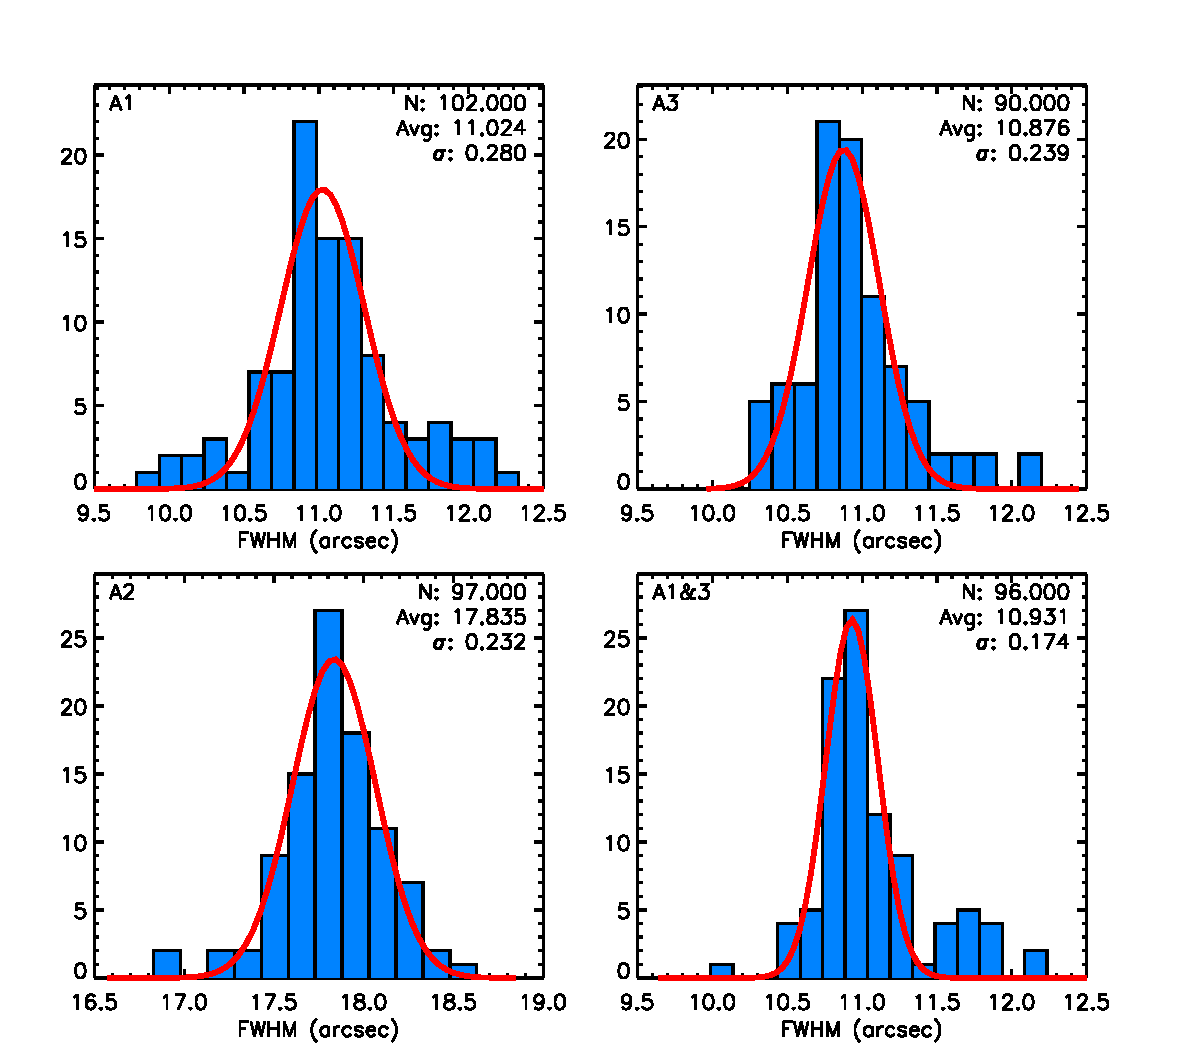
\includegraphics[clip, angle=0, scale=0.7]{Figures/Main_Beam_FWHM_N2R9_10.pdf}
\caption{Distribution of the main beam FWHM estimates using 2D
  Gaussian fits on N2R9 and N2R10 $8' \times 5'$ OTF scans of brigth point sources}
\label{fig:fwhm_map}
\end{center}
\end{figure}

\paragraph{Estimates using beam-map scans}

We use masked version of the beam maps, which are selected as
described in Sect.~\ref{se:beammap_set}. 
Sidelobe masks are defined by a fixed $r_{\rm{out}}$ of $100 arcsec$
and a $r_{\rm{in}}$ that freely varies from $8'$ to $9'$ for the
$260~\rm{GHz}$-arrays, and from $10'$ to $14'$ for the $150~\rm{GHz}$
array. We checked, hovewer, that we obtain consistent results but
larger dispersion when using annulus masks of fixed $r_{\rm{in}}$ of
$8.5'$ and $12'$ at $260$ and $150~\rm{GHz}$ respectively. The median
main beam FWHM and the rms error estimate, which have been obtained
from the nine beam-maps, are given in Table~\ref{tab:fwhm}.

\begin{table}[h]
  \caption[]{FWHM of the NIKA2 main beam in arcsec.}
  \centering
  \begin{threeparttable}
  \begin{tabular}{|l|c|c|c|c|c|}
    \hline
    
       &    &  \multicolumn{4}{|c|}{Array or array combination} \\
    \cline{3-6}
    Method & Dataset        &   A1 &  A3 & A1 $\&$ A3 &  A2  \\
    \hline
    \hline
    Three-Gaussian model G1\tnote{a} &  beam-map &  $10.8 \pm 0.2$  &  $10.8 \pm 0.2$  &  $10.8 \pm 0.3$  &  $17.2 \pm 0.05$  \\
    Sidelobe-masked profile-based    &  TBD      &    &    &    &   \\
    Sidelobe-masked map-based        &  OTF       & $11.0 \pm 0.3$  &  $10.9 \pm 0.2$  &  $11.0 \pm 0.2$  &  $17.8 \pm 0.2$ \\ 
                                     &  beam-map  & $11.3 \pm 0.2$  & $11.2 \pm 0.2$   &  $11.2 \pm 0.2$  &  $17.7 \pm 0.05$ \\ 
    \hline
  \end{tabular}
  \begin{tablenotes}
  \item[(a)] Median FWHM of the first (lowest-FWHM) Gaussian function
    within the Three-Gaussian model fitted from the beam-map scan selection 
  \end{tablenotes}
  \end{threeparttable}
  \label{tab:fwhm}
\end{table}

\subsubsection{FWHM distribution across the FoV}

% COPY FROM THE 'INSTRUMENT' PAPER
\begin{figure}[h]
  \centering
  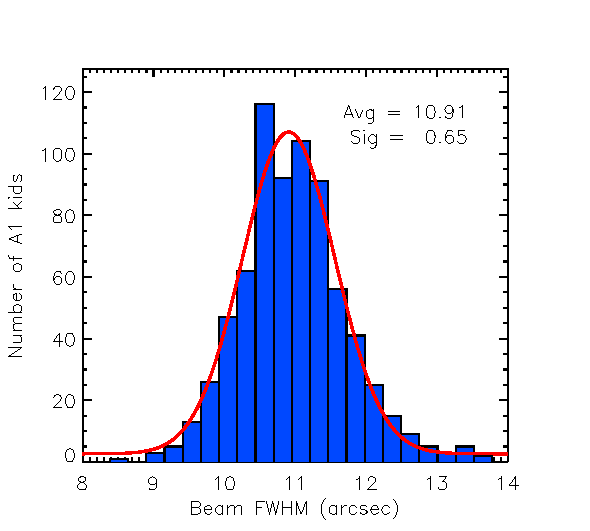
\includegraphics[clip=true,width=0.5\textwidth]{../../../Paper_NIKA2_Technical/plot_histo_A1_fwhm_20170424s123.pdf}
  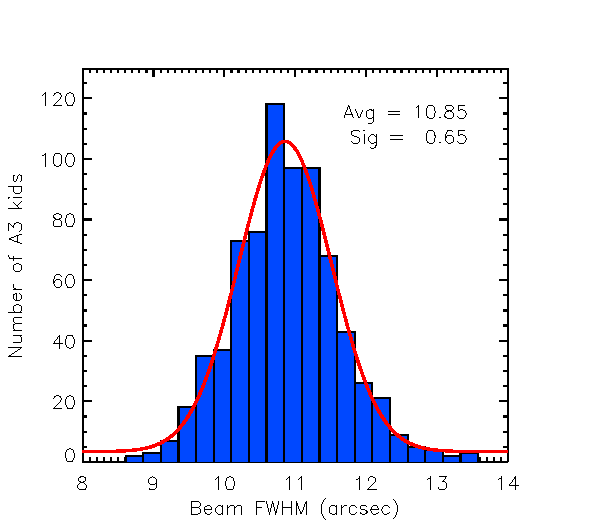
\includegraphics[clip=true,width=0.5\textwidth]{../../../Paper_NIKA2_Technical/plot_histo_A3_fwhm_20170424s123.pdf}
  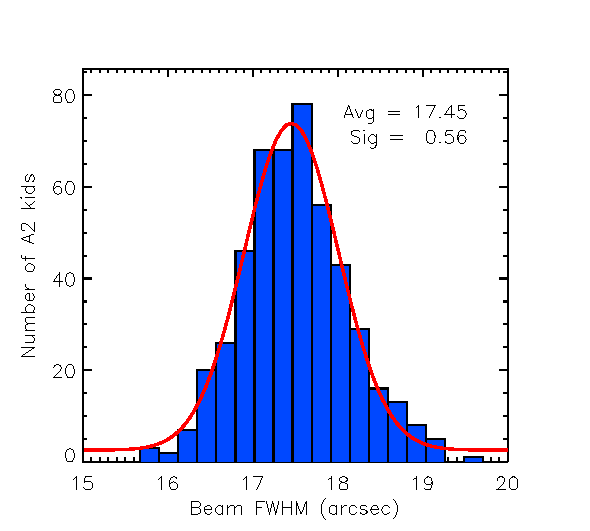
\includegraphics[clip=true,width=0.5\textwidth]{../../../Paper_NIKA2_Technical/plot_histo_A2_fwhm_20170424s123.pdf}
  
\caption{From top to bottom, main beam FWHM distribution of all valid KID detectors of arrays A1, A3, and A2. The main beam FWHM is the geometrical combination of the two-orthogonal FWHM estimates obtained from an elliptical Gaussian fit on side-lobe masked individual maps per KID (see text). The red curves show a Gaussian fit to the histogram data.}
  \label{fig:focalplane_histo}
\end{figure}

Figure \ref{fig:focalplane_histo} shows the distribution of the
main beam FWHMs of the arrays A1, A3 and A2 using a beammap
scan of Neptune acquired during the April 2017 commissioning
campaign and for average weather conditions (scan ID: 20170424s123). We also
show in red the best Gaussian fit to histogram data. We find an
average main beam FWHM of $10.9''$ at 260 GHz and $17.5''$ at
150 GHz in agreement with the main beam estimates gathered in
Table~\ref{tab:fwhm}.
The observed dispersion of about $0.6''$ is expected from the optics desing and its associated
field distortions across the 6.5 arc-minutes FoV, as discussed in
Sect.~\ref{se:grid_distortion}. This quantifies the impact of the
non-constant focus across the FoV, which is characterised in
Sect.~\ref{sec:focus-surf}, on the individual detector main beams.  


\subsection{Beam efficiency}


{\bf discrepant results between methods}


\noindent \emph{method 1:}

Eff = integral of the 2D Gaussian Main Beam / integral of the beam map

\noindent \emph{method 2:}

Eff = integral of the 2D Gaussian Main Beam / integral of the measured profile

\noindent \emph{'Instru' Paper}

Comparing the 2D gaussian main beam fit to the full beam
pattern measurement up to a radius of $250''$, we compute the
beam efficiencies defined as the ratio of power between the main
beam and this full beam. We find beam efficiencies $\approx 55 \%$
and $\approx 75 \%$ for the 260 and 150 GHz channels, respectively.
Heterodyne observations of the lunar edge and of the forward
beam efficiency derived from skydips show that a significant
fraction of the full beam is received from beyond a radius of
$250''$. This fraction is not considered here.


The beam efficiency estimates for the three arrays and the
1mm-array combination are given in Table~\ref{tab:beam_efficiency}.


\begin{table}[h]
  \caption[]{Beam efficiency}
  \centering
  \begin{threeparttable}
  \begin{tabular}{|l|c|c|c|c|}
    \hline
    
       &    \multicolumn{4}{|c|}{Array or array combination} \\
    \cline{2-5}
    Method & A1 &  A3 & A1 $\&$ A3 &  A2  \\
    \hline
    \hline
    2D elliptical-over-deep map beam\tnote{a} &  $0.75 \pm 0.07$  &
    $0.69 \pm 0.04$  &  $0.73 \pm 0.06$  &  $0.85 \pm 0.05$  \\
    2D elliptical-over-measured profile\tnote{a} &  $0.63 \pm 0.10$  &
    $0.56 \pm 0.05$  &  $0.58 \pm 0.06$  &  $0.79 \pm 0.06$  \\
    $250''$ estimates\tnote{b}    &  $0.55$  &   $0.55$ &   $0.55$ &  $0.75$  \\
    \hline
  \end{tabular}
  \begin{tablenotes}
  \item[(a)] Laurence's study
  \item[(b)] values reported in the 'Instrument' paper
  \end{tablenotes}
  \end{threeparttable}
  \label{tab:beam_efficiency}
\end{table}


%% [STABILITY]
%%________________________________________________________
\subsection{Stability of the beam pattern}

\subsubsection{Individual scan beam profiles}

We checked the stability of the beam against various observing
condition (source intensity, weather condition, focus optimisation) by
comparing the beam profile of the beam-map set, which comprizes nine
beam-maps acquired from N2R8 to N2R10, as defined in
Sect.~\ref{se:beammap_set}.
The nine beam profiles and their ratio
w.r.t. the median beam profile are shown in Fig.~\ref{fig:beam_prof}.


\begin{figure}[h]
  \centering
  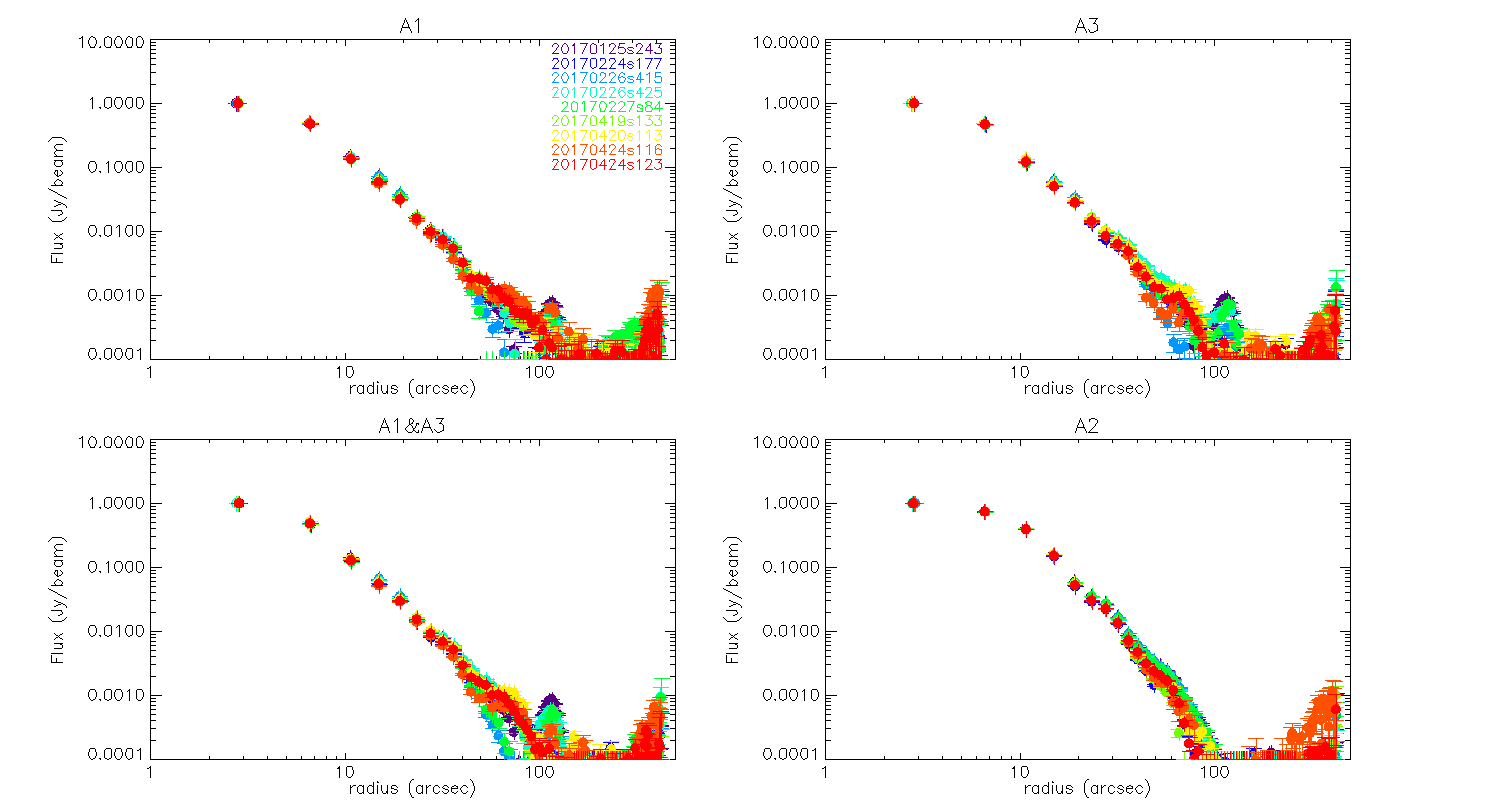
\includegraphics[clip=true,width=\textwidth]{Figures/Profile_allscans_mixed}
  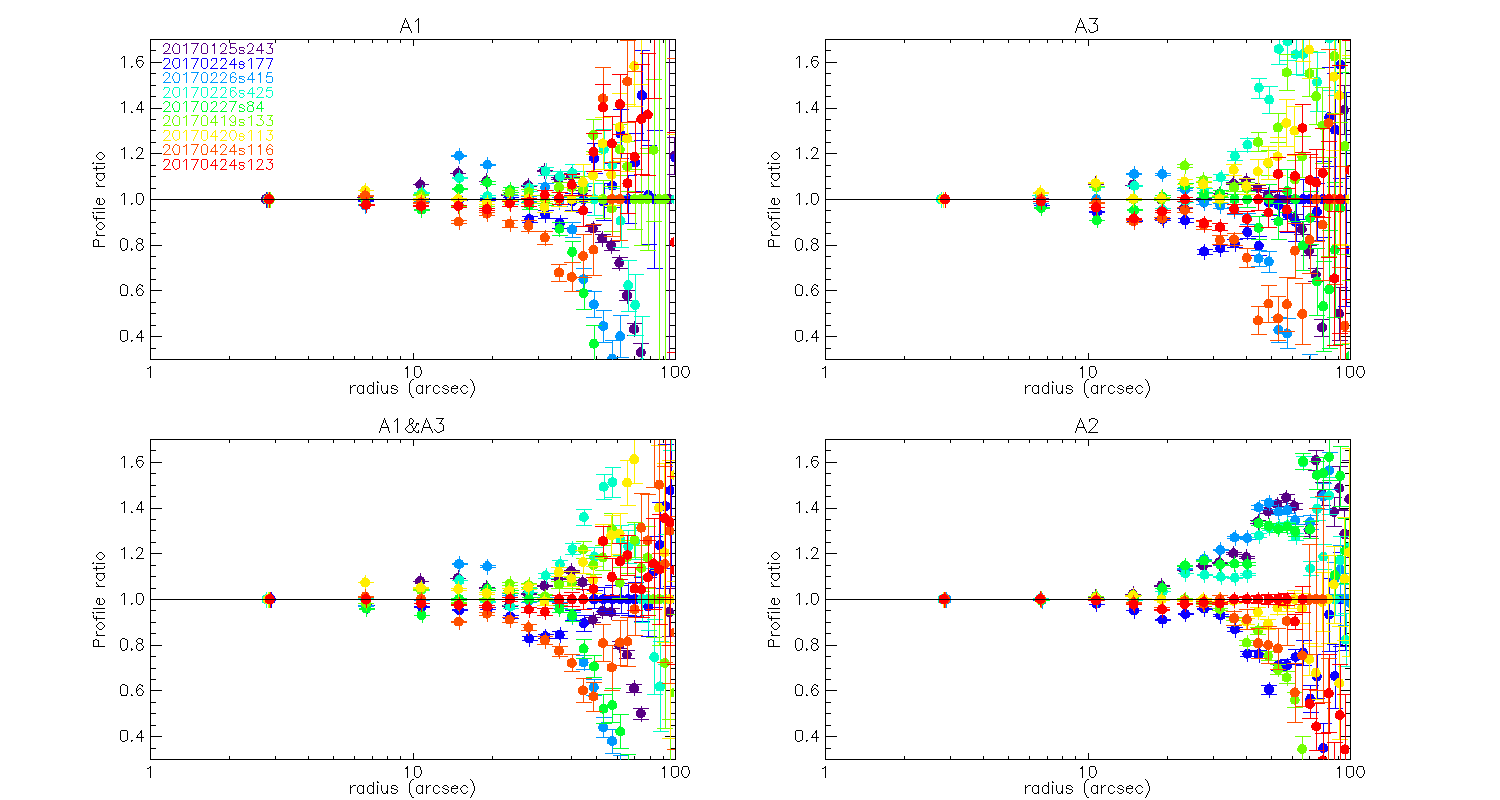
\includegraphics[clip=true,width=\textwidth]{Figures/Profile_allscans_over_median_mixed}
\caption{Stability of the beam profile across various N2R8 to N2R10
  beam-map scans. The upper panel shows the beam profiles normalised
  to the maximum value, and the lower panel the ratios w.r.t. the median profile.}
  \label{fig:beam_prof}
\end{figure}


\subsubsection{Main beam FWHM stability}

[A FAIRE:

  AJOUTER LES PLOTS DE STABILITE EN FONCTION DE ELEVATION, TAU

]



